\chapter{Herramientas y software para la programaci�n en C (entorno GNU/Linux)}

Aunque existen m�ltiples plataformas, mencionamos ahora s�lo las m�s
comunes: Microsoft Windows y GNU/Linux. En Windows disponemos de
herramientas propietarias de desarrollo en C (Microsoft Visual Studio,
Borland, etc) y herramientas de libre distrubuci�n (djgpp, gcc,
etc). Los productos propietarios suelen integrar varias
herramientas en un solo producto IDE\footnote{``suites'' que incorpor�n el
editor, manuales de referencia, compilador....} como Visual Studio, aunque
tambi�n podemos encontrar alg�n IDE de libre distribuci�n. En
cualquier caso, todas las herramientas de libre distrubuci�n que
podamos encontrar para GNU/Linux est�n disponibles para Windows (gcc,
gdb, wincvs, etc).\\

Tambi�n existen IDE's disponibles para GNU/Linux pero en
estas secciones no hablaremos de ellos. Recomendamos en cambio el uso
de las herramientas m�s extendidas y comunes en entornos UNIX. Y de
ellas son de las que hablaremos en las siguientes secciones.
Como es l�gico, la herramienta principal a la hora de programar en
cualquier lenguaje es el compilador (o el int�rprete en su caso). Pero
no es ni mucho menos la �nica herramienta de la que
disponemos. Tambi�n necesitaremos un editor de texto con el que
editaremos el c�digo fuente y, como veremos en este cap�tulo, tambi�n
disponemos de depuradores, sistemas de control de versiones, etc, que
facilitan enormemente la vida del programador.

\section{Compilador: \texttt{gcc}}
GCC\footnote{Originalmente acr�nimo de \textit{GNU C Compiler}. Actualmente se
refiere a \textit{GNU Compiler Collection}, debido a la posibilidad de compilar
otros lenguajes como Ada, Java o Fortran} es un compilador r�pido, muy flexible, y
riguroso con el est�ndar de C ANSI. Como ejemplo de sus m�ltiples
virtudes, diremos que gcc puede funcionar como \textit{compilador
cruzado}\footnote{un compilador cruzado corre bajo una arquitectura,
por ejemplo Intel x86, pero el c�digo binario que genera est� dise�ado
para correr en otra arquitectura distinta, por ejemplo SPARC} para un
gran n�mero de arquitecturas distintas. gcc no proporciona un entorno
IDEs, es solo una
herramienta m�s a utilizar en el proceso. gcc se encarga de realizar (o encargar el 
trabajo a otras utilidades, como veremos) el preprocesado 
(ver \ref{preprocesador}) del c�digo, la compilaci�n,
y el enlazado. Dicho de otra manera, nosotros proporcionamos a gcc
nuestro c�digo fuente en C, y �l nos devuelve un archivo binario
compilado para nuestra arquitectura.\\

Como curiosidad, mencionar que en realidad gcc no genera c�digo
binario alguno, sino c�digo ensamblado. La fase de
ensamblado a c�digo binario la realiza el ensamblador de GNU
(\textit{gas}), y el enlazado de los objetos resultantes, el enlazador
de GNU (\textit{ld}). Este proceso es transparente para el usuario, ya
que a no ser que se lo especifiquemos, gcc realiza el paso desde
c�digo en C a un binario ejecutable autom�ticamente.

\subsection{Manejo de gcc}

Casi siempre, gcc es invocado desde la herramienta \textit{make}, cuyo
funcionamiento se explica m�s adelante. Pero obviamente, debemos saber manejar
m�nimamente gcc para compilar nuestros programas. La sintaxis de gcc es la siguiente:

\begin{verbatim}
Usage: gcc [options] file...
\end{verbatim}

Vamos pues a compilar nuestro primer programa con gcc, que no podr�a
ser de otra manera, ser� un \textit{hola mundo}\footnote{el primer
ejemplo de cualquier tutorial de un lenguaje}:

\ejemplo{herramientas/holamundo.c}

y lo compilamos ejecutando:

\begin{verbatim}
mustang@amarok:~/seminarioc/documentacion/herramientas > gcc holamundo.c 
mustang@amarok:~/seminarioc/documentacion/herramientas > ls
total 68
drwxr-xr-x    4 mustang  mustang      4096 2003-10-30 14:07 .
drwxr-xr-x   16 mustang  mustang      4096 2003-10-30 13:43 ..
-rwxr-xr-x    1 mustang  mustang      5159 2003-10-30 14:00 a.out
-rw-r--r--    1 mustang  mustang        77 2003-10-30 14:00 holamundo.c
mustang@amarok:~/seminarioc/documentacion/herramientas > 
\end{verbatim}

Nos muestra un archivo \verb+a.out+, que es el archivo ejecutable
resultado de la compilaci�n. Lo ejecutamos:

\begin{verbatim}
mustang@amarok:~/seminarioc/documentacion/herramientas > ./a.out 
Hola mundo
mustang@amarok:~/seminarioc/documentacion/herramientas >
\end{verbatim}

Veamos como se comporta si introducimos un error en el fichero:

\ejemplo{herramientas/holamundo_error.c}

\begin{verbatim}
mustang@amarok:~/seminarioc/documentacion/herramientas > gcc holamundo_error.c
holamundo_error.c: In function `main':
holamundo_error.c:7: `a' undeclared (first use in this function)
holamundo_error.c:7: (Each undeclared identifier is reported only once
holamundo_error.c:7: for each function it appears in.)
holamundo_error.c:7: parse error before `return'
mustang@amarok:~/seminarioc/documentacion/herramientas >
\end{verbatim}

Como vemos gcc  nos proporciona el fichero y la l�nea en la que ha
detectado el error. El formato de la salida de error es reconocido por
la mayor�a de los editores, que nos permiten visitar esa posici�n con
atajos de teclado\footnote{en el editor Emacs, se puede hacer
  compilando mediante M-x compile, y usando el atajo C-x \`\
  SPC}. Obviamente, cuando gcc genera alg�n error, no se crea archivo
ejecutable como resultado.

\subsection{Warnings y errores}

\definicion{Error}{fallo al analizar el c�digo C que impide la
generaci�n de un ejecutable final.}

\definicion{\textit{Warning}}{advertencia del compilador al analizar
  el c�digo C que no impide la generaci�n de un ejecutable
  final.} 

Vamos a provocar que gcc se queje con un \textit{warning}. Para ello,
utilizamos el siguiente c�digo:

\ejemplo{herramientas/holamundo_warning.c}

Y lo compilamos con:

\begin{verbatim}
mustang@amarok:~/documentacion/herramientas > gcc -Wall holamundo_warning.c
holamundo_warning.c: In function `main':
holamundo_warning.c:6: warning: control reaches end of non-void function
mustang@amarok:~/documentacion/herramientas >
\end{verbatim}

\begin{flushleft}
A pesar del \textit{warning}, gcc ha compilado un fichero ejecutable. M�s
adelante veremos el significado de la opci�n \verb+-Wall+.
\end{flushleft}



\subsection{Opciones m�s comunes}

\label{opciones_gcc}

A continuaci�n mostramos algunas de las opciones m�s habituales al
usar gcc:

\begin{itemize}

\item{\texttt{--help}}

Indica a gcc que muestre su salida de ayuda (muy reducida).

\item{\texttt{-o <file>}}

El archivo ejecutable generado por gcc es por defecto \verb+a.out+. Mediante
este modificador, le especificamos el nombre del ejecutable. 

\item{\texttt{-Wall}}

No omite la detecci�n de ning�n warning. Por defecto, gcc omite una
colecci�n de warnings ``poco importantes''.

\item{\texttt{-g}}

Incluye en el binario informaci�n necesaria para utilizar un depurador
posteriormente. 

\item{\texttt{-O <nivel>}}

Indica a gcc que utilice optimizaciones en el c�digo. Los niveles
posibles van desde 0 (no optimizar) hasta 3 (optimizaci�n
m�xima). Utilizar el optimizador aumenta el tiempo de compilaci�n,
pero suele generar ejecutables m�s r�pidos.

\consejo{No utilices optimizaci�n cuando generes un ejecutable con informaci�n
de depuraci�n (opcion \texttt{-g}). Las optimizaciones introducidas pueden
confundir al depurador.}

\item{\texttt{-E}}

S�lo realiza la fase del preprocesador, no compila, ni ensambla, ni
enlaza.

\item{\texttt{-S}}

Preprocesa y compila, pero no ensambla ni enlaza.

\item{\texttt{-c}}

Preprocesa, compila y ensambla, pero no enlaza.

\item{\texttt{-I <dir>}}

Especifica un directorio adicional donde gcc debe buscar los archivos
de cabecera indicados en el c�digo fuente (ver \ref{include}).

\item{\texttt{-L <dir>}}

Especifica un directorio adicional donde gcc debe buscar las librer�as
necesarias en el proceso de enlazado (ver \ref{enlazado}).

\item{\texttt{-l<library>}}

Especifica el nombre de una librer�a adicional que deber� ser
utilizada en el proceso de enlazado (ver \ref{enlazado}).

\end{itemize}

La colecci�n completa de modificadores a utilizar con gcc se encuentra
en su p�gina de manual, \verb+man gcc+, cuyo manejo se explica un poco
m�s adelante (ver \ref{man}).


\section{Depuradores: \texttt{gdb} y \texttt{ddd}}
\label{gdb}

\definicion{Depurador}{Herramienta que permite al programador seguir la
ejecuci�n de su programa paso a paso, as� como ver el contenido de variables.}

\subsection{Depurando con \texttt{gdb}}

Para poder ejecutar un depurador sobre nuestros programas en C,
debemos especificar a gcc que incluya informaci�n de depuraci�n en los
binarios que genere. Como se vio en \ref{opciones_gcc}, en el caso de utilizar
gcc compilamos el programa 
con el modificador \texttt{-g}. 

\subsection{Depurador gr�fico: \texttt{ddd}}

DDD es un interfaz gr�fico para el depurador gdb. La principal ventaja
de ddd es la facilidad para mostrar los contenidos de las posiciones
de memoria durante la ejecuci�n de nuestro programa, como puede verse
en la siguiente captura:

\begin{figure}[H]
\begin{centering}
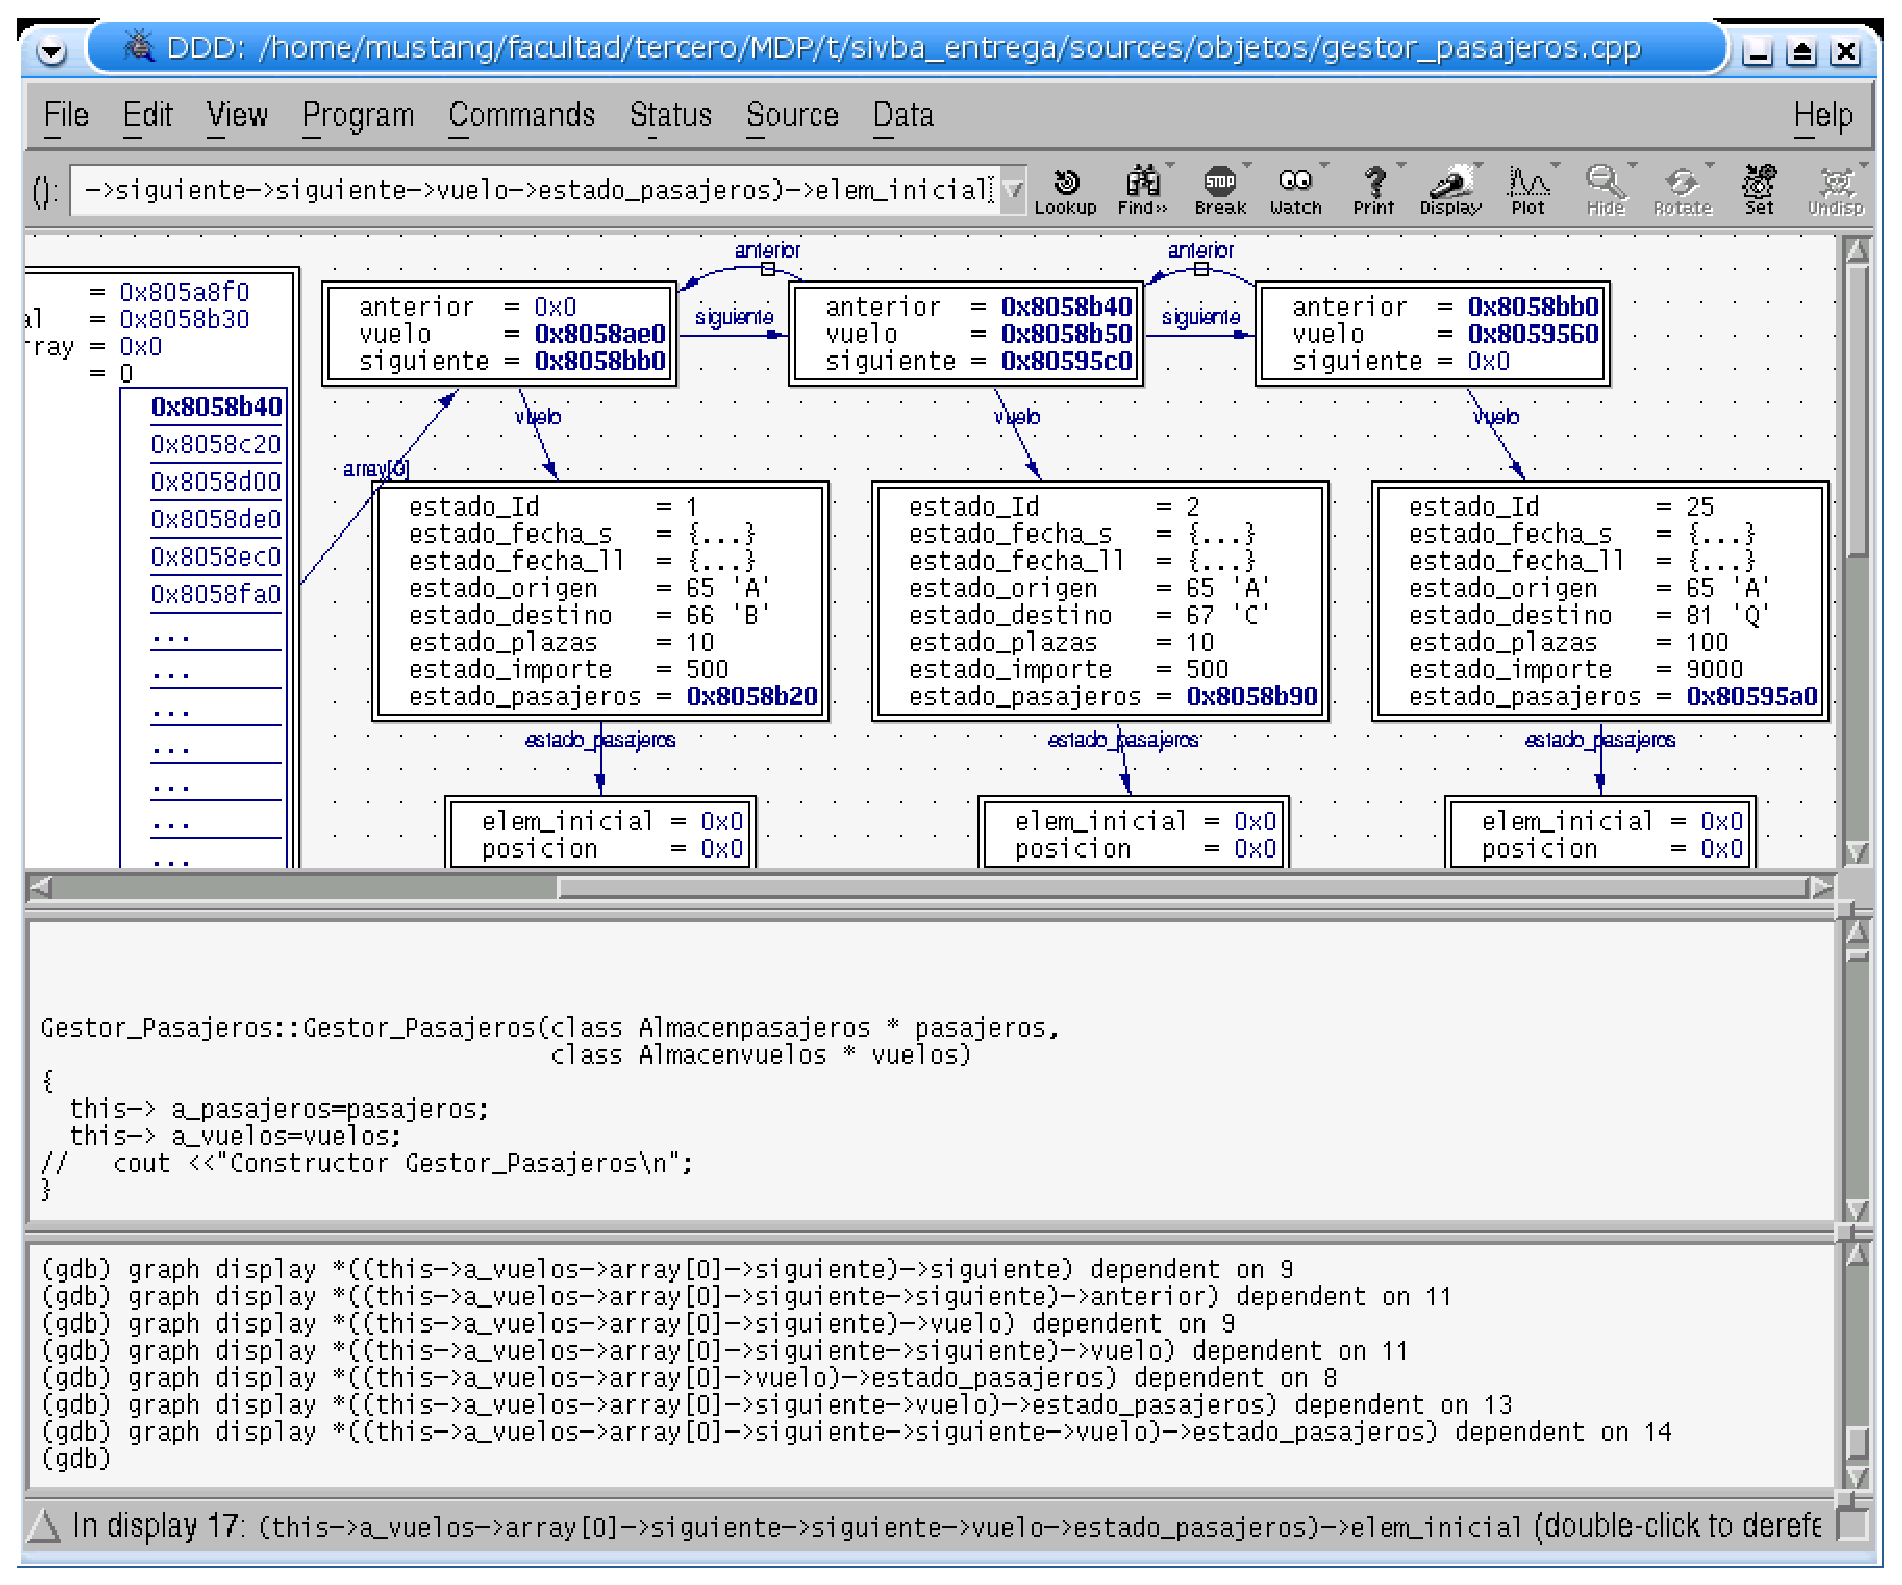
\includegraphics[width=18cm]{herramientas/ddd.eps}
\caption{DDD en accion, cadenas enlazadas}
\end{centering}
\end{figure}

\subsection{Manejo}

Para obtener una descripci�n del manejo de gdb y ddd, os remitimos a
la documentaci�n de un seminario previo de ACM: \cite{Adan}.


\section{Control de dependencias: \texttt{make}}
La mayor�a de nuestros proyectos de programaci�n
no constar�n de un solo fichero fuente sino de varios (puede
incluso que de centenas de ellos). Cuando editamos un fichero de c�digo
fuente y lo modificamos pasamos a compilarlo (con GCC o cualquier otro
compilador). Hay tener en cuenta que puede haber otros ficheros de
c�digo fuente que dependan del que acabamos de modificar. Por lo tanto, esos
ficheros de c�digo fuente que dependen del que acabamos de modificar
tambi�n deben ser compilados. La herramienta make nos evita la tediosa
tarea de compilar las dependencias, por no hablar de que nos
evita la necesidad de tener presente en todo momento cuales son las
dependencias entre ficheros de c�digo fuente. Para ello nos valemos de
un fichero (t�picamente con nombre \texttt{Makefile}) en el que
declaramos las dependencias entre ficheros de c�digo fuente y las
�rdenes necesarias para actualizar cada fichero. Una vez escrito el
fichero \texttt{Makefile}, cada vez que cambiemos alg�n fichero
fuente, con la orden:
\begin{verbatim}
make
\end{verbatim}
basta para que se realicen todas las recompilaciones necesarias.
Veamos ahora el formato b�sico del fichero \texttt{Makefile}.
El fichero Makefile m�s simple est� compuesto por ``reglas'' de este
aspecto.
\begin{verbatim}
objetivo ... : prerrequisitos ...
            comando
            ...
            ...
\end{verbatim}

Un objetivo suele ser el nombre de un fichero generado por un
programa; ejemplos de objetivos son ficheros ejecutables u objetos. Un
objetivo puede ser tambi�n el nombre de una acci�n a llevar a cabo,
como ``clean'', que veremos m�s adelante en un ejemplo.\\

Un prerrequisito es un fichero que se usa como entrada para crear un
objetivo. Un objetivo con frecuencia depende de varios ficheros.\\

Un comando es una acci�n que \texttt{make} ejecuta. Una regla puede
tener m�s de un comando, cada uno en su propia
l�nea. \emph{\bf{Atenci�n}:} �hay que poner un tabulador al
principio de cada l�nea de comando!\\

Normalmente un comando est� en una regla con prerrequisitos y
contribuye a crear un fichero objetivo si alguno de los prerrequisitos
cambia. Un ejemplo de excepci�n a esto es el objetivo ``clean'', que no
tiene prerrequisitos. Una regla, por tanto, explica como y cuando
reconstruir ciertos ficheros que son objetivos de reglas.\\

A continuaci�n tenemos un ejemplo de un Makefile que describe la manera en la
que un fichero ejecutable llamado ``edit'' depende de ocho
ficheros objeto que a su vez dependen de ocho ficheros de c�digo
fuente C y tres archivos de cabecera. Los ocho ficheros de c�digo
fuente C dependen del archivo de cabecera ``defs.h'' (como dijimos
anteriormente, mediante la directiva \texttt{\#include}). S�lo los
ficheros de c�digo que definen los comandos de edici�n dependen de
``command.h'', y s�lo los ficheros de operaciones de bajo nivel que
cambian el buffer del editor dependen de ``buffer.h''.

\begin{verbatim}
edit: main.o kbd.o command.o display.o \
      insert.o search.o files.o utils.o
       gcc -o edit main.o kbd.o command.o display.o \
             insert.o search.o files.o utils.o

main.o : main.c defs.h
       gcc -c main.c

kbd.o : kbd.c defs.h command.h
       gcc -c kbd.c

command.o : command.c defs.h command.h
       gcc -c command.c

display.c : display.c defs.h buffer.h
       gcc -c display.c

insert.o : insert.c defs.h buffer.h
       gcc -c insert.c

search.o : search.c defs.h buffer.h
       gcc -c search.c

files.o : files.c defs.h buffer.h command.h
       gcc -c files.c

utils.o : utils.c defs.h
       gcc -c utils.c

clean :
       rm -f edit *.o

\end{verbatim}

En el ejemplo dividimos cada l�nea larga en dos l�neas usando la
contrabarra\footnote{El car�cter $\backslash$}. Para crear el fichero ejecutable
  ``edit'', escribimos: 
\begin{verbatim}
make
\end{verbatim}
Para borrar el fichero ejecutable y todos los ficheros objeto del
directorio, escribimos:
\begin{verbatim}
make clean
\end{verbatim}

En el fichero Makefile del ejemplo, son objetivos el fichero
ejecutable ``edit'' y los ficheros objeto ``main.o'' y ``kbd.o'', entre
otros. Son prerrequisitos ficheros como ``main.c'' y ``defs.h''. De hecho,
cada fichero ``.o'' es tanto objetivo como prerrequisito. Son comandos
``gcc -c main.c'' y ``gcc -c kbd.c''.\\

Cuando un objetivo es un fichero, necesita ser recompilado si
cualquiera de los prerrequisitos cambia. Adem�s, cualquier
prerrequisito que es generado autom�ticamente deber�a ser actualizado
primero. En el ejemplo, ``edit'' depende de cada uno de los ocho
ficheros objeto; el fichero objeto ``main.o'' depende a su vez del fichero de
c�digo fuente ``main.c'' y del fichero de cabecera ``defs.h''. \\

Un comando de shell sigue a cada l�nea que contiene un objetivo y
prerrequisitos. Estos comandos de shell indican como actualizar el
fichero objetivo. Recuerda que hay que poner un tabulador al principio
de cada l�nea de comando para distinguir l�neas de comando de otras
l�neas en el Makefile. (Ten en cuenta que \texttt{make} no sabe nada
sobre c�mo funcionan los comandos. Depende de t� proporcionar los
comandos que actualizaran los ficheros objetivos de manera apropiada).\\

El objetivo ``clean'' no es un fichero, es simplemente el nombre de una
acci�n. Tampoco es un prerrequisito de otra regla ni tiene
prerrequisitos. Por tanto, \texttt{make} nunca har� nada con este
objetivo a no se que se le pida espec�ficamente.\\

Con esto hemos visto el funcionamiento m�s esencial de la herramienta
\texttt{make}. Pero \texttt{make} es mucho m�s. En la bibliograf�a
podemos encontrar referencias a documentaci�n m�s extensa de
\texttt{make}. 


\section{Manuales: \texttt{man}}
\label{man}

\verb+man+\footnote{El nombre del comando viene de \texttt{manual}} es un mandato de Unix/Linux que nos informa sobre el funcionamiento de
otros mandatos.
El funcionamiento de man no s�lo se limita a informarnos sobre el uso
de mandatos, nos informa tambi�n de funciones de libreria y llamadas a
funciones del sistema. Los archivos de manual de \verb+man+ se encuentran organizados en 9 secciones, de
las cuales, ahora s�lo estamos interesados en las 3 primeras:\\

\begin{tabular}{c|l}
\textbf{Secci�n} & \textbf{Descripci�n} \\
\hline
      1 &  Programas ejecutables y comandos de la shell \\
          \hline
       2 &  Llamadas al sistema\\
           \hline
       3  & Llamadas a funciones de biblioteca \\
           \hline
\end{tabular}
\vspace{0.4cm}
%\begin{flushleft}
%Existen 6 secciones m�s pero no nos interesan para la programaci�n en C.
%\end{flushleft}

Antes de comenzar a utilizar  \verb+man+ es recomendable que nos informemos m�s
sobre su utilizaci�n (\verb+man man+).
Aqui encontraremos algunas opciones muy �tiles:\\

\begin{tabular}{c|l}
\textbf{Opci�n} & \textbf{Descripci�n} \\
\hline
     -a &  Muestra de forma consecutiva las secciones en que existe manual del comando \\
     \hline
     -k &  Muestra las paginas de manual y secciones en que se hace referencia a lo buscado \\
     \hline
\end{tabular}
\vspace{0.4cm}

En el momento de buscar informaci�n 
debemos tener en cuenta que algunas funciones y
mandatos se encuentran en varias secciones 
y, por lo tanto, deberemos indic�rselo al man antes de su ejecuci�n. Para
especificar la secci�n sobre la que queremos consultar, lo haremos de la
siguiente forma: 
\begin{verbatim}
        man [n� seccion] [mandato]
\end{verbatim}


Como ejemplo de la utilizaci�n de \verb+man+, consultemos el uso de printf como llamada a funci�n de biblioteca, mediante la siguiente linea:
\begin{verbatim}
        man 3 printf
\end{verbatim}

Ahora veamos su uso como comando de la Shell:
\begin{verbatim}
        man 1 printf
\end{verbatim}





\section{Control Concurrente de Versiones: \texttt{cvs}}

CVS significa \textit{Concurrent Version System}. Es una herramienta
que nos permite mantener nuestro trabajo en un \textbf{repositorio},
al que m�ltiples usuarios pueden conectarse y realizar cambios. En
nuestra opini�n, es una de las mejores ayudas para el trabajo en
equipo, e incluso, para el trabajo individual (control de cambios en
las versiones). 

\subsection{Escenario de uso}

El usuario crea un repositorio en una m�quina, que almacenar� el
proyecto en el que se va a trabajar. Cada vez que se crea un archivo
nuevo en el proyecto, o un subdirectorio, se introduce en el repositorio
con un n�mero de versi�n inicial. Una vez creado el repositorio, cada usuario puede conectarse con el
servidor y descargarse una copia del mismo a su m�quina, trabajar con
los ficheros, y enviar los cambios al servidor. \\

Donde se nota realmente la potencia del sistema es cuando los
usuarios trabajan sobre los mismos ficheros. Mientras los cambios sean
en zonas diferentes de un mismo fichero, CVS se encarga de mezclar las
versiones sin interacci�n del usuario. El �nico escenario que requiere
intervenci�n del usuario es el siguiente:

\begin{itemize}
\item el usuario A se descarga la versi�n 1.3 del fichero X
\item el usuario B se descarga la versi�n 1.3 del fichero X
\item el usuario A modifica el fichero X y lo sube, generando la
  versi�n 1.4
\item el usuario B modifica el fichero X en el mismo sitio y lo sube,
  produciendo un conflicto con los cambios del usuario A
\end{itemize}

En este caso, CVS avisa al usuario B de que tiene que reconciliar a
mano ambas versiones, y le proporciona las diferencias entre sus
modificaciones y las de su compa�ero. Una vez que el usuario B corrige
a mano esos cambios, sube el fichero, generando la version 1.5.\\

CVS proporciona otras muchas ventajas, como poder generar ramas a
partir de un punto del proyecto, permitiendo que los usuarios trabajen
en ramas distintas, y muy importante, permite recuperar cualquier
versi�n de cualquier archivo existente. Podemos, por ejemplo,
recuperar un archivo tal y como estaba hace un mes.\\

A continuaci�n se muestra un ejemplo de operaci�n sobre un
repositorio:

\begin{verbatim}
Borrado gdb.tex, ya no era necesario
Cambios en las tildes de cvs.
CVS: ----------------------------------------------------------------------
CVS: Enter Log.  Lines beginning with `CVS:' are removed automatically
CVS: 
CVS: Committing in .
CVS: 
CVS: Modified Files:
CVS:    cvs.tex 
CVS: Removed Files:
CVS:    gdb.tex 
CVS: ----------------------------------------------------------------------
\end{verbatim}


\subsection{Manejo}

Os remitimos a la estupenda documentaci�n realizada por un compa�ero
de ACM en \cite{Hernando}.


\section{Herramientas de desarrollo C sobre Windows}

Cuando utilizamos Windows no tenemos tan claro que compilador utilizar
ya que en Windows disponemos de herramientas portadas de Linux
(gcc.exe) o las herramientas que Microsoft nos proporciona para
desarrollar programas (Visual Studio) que podemos obtener de
Biblioteca con una licencia de estudiante de forma gratuita.

\subsection{GCC en Windows}

La compilaci�n de un programa utilizando el GCC se realiza de la misma
forma a la vista en Linux, pero debemos tener en cuenta que no todo
programa que compile en Linux compila en Windows debido a las
diferencias existentes en las llamadas al sistema. Esto es debido a  que Windows
no cumple completamente con el estandar POSIX (ver \ref{posix}) de llamadas al sistema. 
Estas
herramientas para Windows las podemos obtener por medio de diferentes
programas, ya sea bajandonos el conjunto de herramientas UNIX para
Windows \textit{MinGW}, o descarg�ndonos desde la facultad el compilador
de Ada95 \textit{(GNAT)}, el cual viene con un el GCC, ya que la
compilaci�n llevada a cabo por \textit{GNATMAKE} es una traducci�n del
lenguaje Ada a C y una posterior compilaci�n en C.  Estas herramientas
estan disponibles desde las siguientes direcciones:

\begin{itemize}
\item \url{ftp://lml.ls.fi.upm.es/pub/lenguajes/ada/gnat/3.13p/winnt/}
\item \url{http://www.mingw.org/download.shtml}
\end{itemize}

%Si nos decantamos por la utilizaci�n del GCC proporcionado por \textit{GNATMAKE} deberemos
%tener en cuenta que los programas que queramos compilar deben ser copiados a la ruta ...
Y recordad, tanto si elegimos utilizar el paquete de utilidades Linux
que encontramos en \textit{MinGW}, como si elegimos el \textit{GNAT},
deberemos incluir la ruta donde instalemos estos archivos en nuestro
\verb+PATH+ para que funcione la compilaci�n. Otra posibilidad es
crear todos los archivos dentro de la carpeta donde se encuentre
instalado \textit{MinGW} o el archivo \verb+gcc.exe+ ya que en caso
contrario, Windows no podra localizar el compilador \verb+gcc+ y nos
mostrara ese maravilloso mensaje de error:

\begin{verbatim}
"gcc" no se reconoce como un comando interno o externo, programa o
archivo por lotes ejecutable.
\end{verbatim}

% \subsection{Visual Studio}
% 
% Si decidimos utilizar como herramienta de compilaci�n este programa,
% nos encontraremos con un interfaz de desarrollo orientado a proyectos
% con C++ pero podremos utilizarlo tambien para compilar nuestros
% programas en C.
% 
% Tambi�n mencionaremos aqu� la depuraci�n disponible en Visual Studio,
% el cual nos permitira visualizar los valores de las direfentes
% variables, desde su valor en memoria y la ejecuci�n paso a paso de
% cada una de las lineas de c�digo.
% 
% \subsection{Depuracion: \texttt{gdb}}
% 
% En Windows, al igual que pasaba con el gcc, disponemos de un GDB
% portado desde Linux, el cual funciona de identica manera a la
% explicada en la secci�n \ref{gdb}.

